%% =====================================================================
%%  PetSafe-Greenery -- final report skeleton
%%  COMP5511: Artificial Intelligence Concepts
%%
%%  Format requirements imposed by the course:
%%    A4, 12 pt Times New Roman, 2.5 cm margins on all four sides,
%%    single line spacing, 1-page cover, at most 10 pages of content,
%%    references are unlimited.
%%
%%  HOW TO USE THIS FILE
%%    1.  Every  TODO  marker is a place you must fill in with your own
%%        text / your own measured numbers.
%%    2.  Do not paste real source code into the report -- the course
%%        explicitly asks for pseudocode (Algorithm 1/2 below).
%%    3.  Copy the measured numbers straight out of
%%        results/runs/<provider>__<model>/summary.csv.
%%    4.  Compile twice so that the cross-references resolve.
%% =====================================================================
\documentclass[12pt,a4paper]{article}

\usepackage[T1]{fontenc}
\usepackage{mathptmx}   % Times-like serif (portable; requires only base psnfss)
\usepackage[margin=2.5cm]{geometry}    % 2.5 cm on all four sides
\usepackage{setspace}
\usepackage{graphicx}
\usepackage{booktabs}
\usepackage{amsmath}
\usepackage{amssymb}
\usepackage{xcolor}
\usepackage{graphicx}
\graphicspath{{figures/}{../figures/}}
\usepackage{enumitem}
\usepackage[hidelinks]{hyperref}

\setstretch{1.0}                      % single line spacing
\setlist{nosep,leftmargin=*}
% --- tight float spacing (keeps 10 content pages + cover + references) --- %
\setlength{\textfloatsep}{12pt plus 2pt minus 2pt}
\setlength{\floatsep}{10pt plus 2pt minus 2pt}
\setlength{\intextsep}{10pt plus 2pt minus 2pt}
\setlength{\abovecaptionskip}{5pt}
\setlength{\belowcaptionskip}{0pt}
\setlength{\abovedisplayskip}{6pt plus 2pt minus 2pt}
\setlength{\belowdisplayskip}{6pt plus 2pt minus 2pt}
\renewcommand{\topfraction}{0.9}
\renewcommand{\bottomfraction}{0.7}
\renewcommand{\textfraction}{0.08}
\renewcommand{\floatpagefraction}{0.75}
\pagestyle{plain}

\newcommand{\todo}[1]{\textcolor{red}{\textbf{[TODO: #1]}}}
\newcommand{\metric}[1]{\textbf{#1}}

\title{\vspace{1.2cm}\textbf{PetSafe-Greenery: A Dual-Constraint Agentic Workflow for\\
Pet-Friendly Balcony and Courtyard Planting Design}\\[0.6cm]
\normalsize COMP5511: Artificial Intelligence Concepts --- Final Project Report}
\author{Student Name: CHEN Niannian \qquad Student ID: 26063619G}
\date{}

\begin{document}

% ------------------------------------------------------------------ cover
\begin{titlepage}
  \thispagestyle{empty}
  \begin{center}
    \vspace*{1.5cm}
    {\LARGE \bfseries PetSafe-Greenery: A Dual-Constraint Agentic Workflow for\\[0.3cm]
    Pet-Friendly Balcony and Courtyard Planting Design\par}
    \vspace{1.5cm}
    {\large COMP5511: Artificial Intelligence Concepts\par}
    \vspace{0.4cm}
    {\large Final Project Report\par}
    \vfill
    {\large Student Name: CHEN Niannian\par}
    \vspace{0.2cm}
    {\large Student ID: 26063619G\par}
    \vspace{1cm}
    {\large The Hong Kong Polytechnic University\par}
  \end{center}
\end{titlepage}

\section{Motivation}

Urban pet ownership is rising, and so is the number of balconies and private
courtyards that people want to turn into gardens. The obstacle is that the
ornamental-plant trade and the pet-toxicology literature overlap far more than
laypeople expect: hundreds of common ornamental species contain compounds that
are hazardous to companion animals. True lilies (\textit{Lilium} spp.) induce
acute, fatal renal failure in cats even when only pollen is ingested;
\textit{Cycas revoluta} (sago palm) causes hepatic failure through the alkaloid
cycasin; and ubiquitous foliage plants such as pothos
(\textit{Epipremnum aureum}) and peace lily (\textit{Spathiphyllum}) cause
intense oral irritation from calcium oxalate rasters.

The difficulty is that this is not a single-constraint problem. A scheme must
simultaneously satisfy two independent constraint families: a
\emph{microclimate} constraint (sunlight exposure, soil moisture, container
depth) and a \emph{veterinary safety} constraint (non-negotiable). Foundation
LLMs fail on this task in a characteristic way. Asked for a cat-friendly
sunny balcony, they will happily propose pothos, sago palm or true lilies,
because those species are salient in their training data and because the
instruction "make it pet-safe" is a soft preference that competes with
"make it look beautiful". They will also cheerfully place sun-loving plants
in a north-facing balcony receiving no direct light at all, which kills the
plants.

These two failures have a common structure: they are both \emph{constraint
violations}, and both are failures of the same kind --- the model must recall
and apply a fact that lives outside its parametric memory (a toxicity label,
a light tolerance) and that it cannot check for itself. This motivates the
central question of this project:

\begin{quote}
\textit{If a constraint can be checked deterministically, should an LLM be
allowed to decide it?}
\end{quote}

\textbf{Intended users.} Pet-owning apartment residents without horticultural
training; landscape-architecture and horticulture students who need a safe,
defensible first draft; and junior planting designers who must justify every
species to a client who owns a cat.

Our approach answers the question affirmatively. We build a multi-tool agentic
workflow in which the LLM is responsible only for what it is good at ---
reading a brief and composing a spatially organised design --- while every
safety-critical decision is delegated to a deterministic Python filter over a
curated ground-truth database. The workflow is evaluated against two baselines
on twenty-five benchmark scenarios.

\section{Description}

\subsection{The workflow}

Figure~\ref{fig:workflow} summarises the system.

\begin{figure}[t]
  \centering
  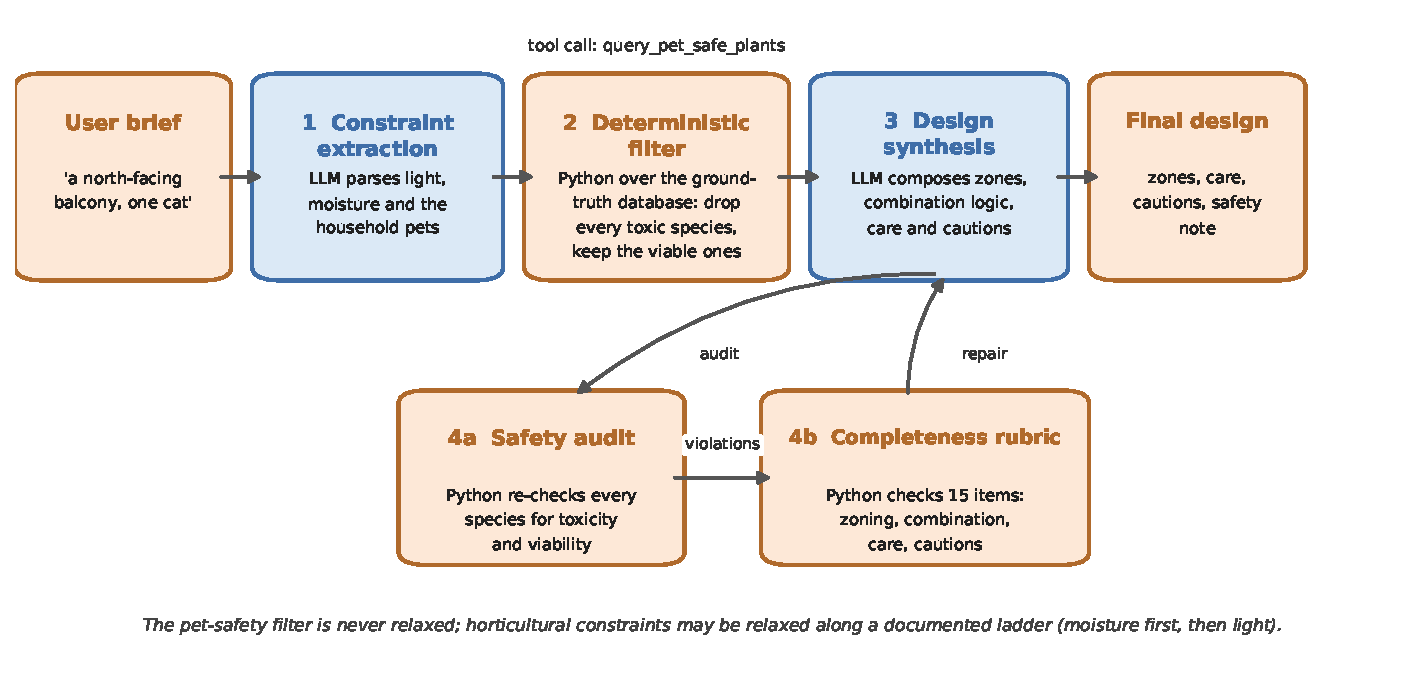
\includegraphics[width=0.80\linewidth]{fig_workflow.pdf}
  \caption{The dual-constraint agentic workflow. Solid boxes are LLM stages,
  dashed boxes are deterministic Python stages. The pet-safety filter is never
  relaxed; horticultural constraints may be relaxed along a documented ladder.}
  \label{fig:workflow}
\end{figure}

\textbf{Stage 1 --- Multi-constraint extraction.} The model parses the user's
natural-language brief into structured parameters: the microclimate (a light
class in \{full\_sun, partial\_shade, bright\_indirect, full\_shade\}, a
moisture class in \{low, moderate, high\}) and the household pet profile
(cat / dog / both / none).

\textbf{Stage 2 --- Deterministic tool execution.} Instead of recalling
toxicity from parametric memory, the model calls the tool
\texttt{query\_pet\_safe\_plants}, implemented in Python over a curated
ground-truth database. The tool (i) removes every species toxic to any
household pet, (ii) keeps only species whose light and moisture requirements
match the site, and (iii) returns the surviving candidate pool. Because the
filter is a set operation over an explicit table, the stage cannot
hallucinate and its result is auditable species by species.

\textbf{Stage 3 --- Dual-constraint synthesis.} The model composes the final
scheme from the verified candidates only. A planting scheme is not a list of
species, so the output contract obliges the model to produce four things
beyond the species themselves:

\begin{enumerate}[leftmargin=1.5em]
  \item \emph{Spatial structure.} 2--4 zones stacked in height, using an
    explicit three-layer taxonomy: \emph{vertical} (trailing or hanging
    plants above eye level), \emph{mid} (upright plants at knee-to-waist
    height) and \emph{ground} (low planting or edging at floor level). Exactly
    one zone must be pet-accessible (role \texttt{grazing}), i.e.\ a spot the
    animal can reach. Each zone carries its own layer, placement and light
    position.
  \item \emph{Combination logic.} \texttt{layout\_strategy} (how the layers
    stack and how the eye moves through the space), \texttt{combination\_logic}
    (the contrast in height, texture, leaf shape, colour, scent and seasonal
    rhythm), and a per-plant \texttt{role\_in\_combination} stating what that
    plant contributes and how it interacts with its neighbours.
  \item \emph{Care.} Per-zone \texttt{maintenance} entries and a site-wide
    \texttt{care\_instructions} list in which every entry states what to do,
    how often and in which season.
  \item \emph{Care cautions.} \texttt{care\_cautions}: what actually goes
    wrong with \emph{this} scheme --- overwatering in the hanging baskets,
    scorch on a hot west wall, frost damage to tender perennials, a plant the
    pet will chew, poor drainage in the corner pot.
\end{enumerate}

All three evaluated methods receive exactly this contract, so the comparison
measures the architecture (grounding and filtering), not the prompt: asking
less of the baselines would confound the two.

\textbf{Stage 4a --- Self-correction / audit loop.} A deterministic auditor
re-checks every recommended species against the database for toxicity and
viability. If any violation survives, the model receives the explicit list of
violations and one repair opportunity; the repaired design is audited again.
The agent is therefore fail-safe rather than fail-silent: even a model that
ignores its instructions cannot emit an unsafe recommendation without the
violation being detected and reported.

\textbf{Stage 4b --- Completeness repair loop.} Correct species are
necessary but not sufficient for a useful scheme. A second deterministic
rubric checks whether the design actually contains the spatial structure, the
combination logic, the care instructions and the care cautions it promises
(Section~\ref{sec:rubric}). Missing items are listed back to the model, which
gets one repair round --- the same mechanism that closes the loop on safety
now closes it on design quality: a checkable property is verified by code,
and the model is asked to fix what the check found.

\subsection{Constraint relaxation ladder}

A strict filter can return an empty pool when the database happens to contain
no species for an unusual combination of conditions. Rather than returning
nothing, the tool relaxes \emph{horticultural} constraints along a fixed
ladder --- first moisture, then light --- and reports the relaxation level
back to the agent, which must then tell the user that the site is marginal.
The \emph{pet-safety} filter is never relaxed at any level. This asymmetry is
the core safety argument of the project and is visible in the tool output.

\subsection{Models, tools and why this design}

We call a hosted chat-completions API with function calling. The
implementation supports two interchangeable providers, selected by one
environment variable: Google AI Studio (Gemini) and DeepSeek, which speaks
the OpenAI-compatible protocol. The provider and the exact model are written
into every result file and into the run's \texttt{usage.json}, so every number
in this report can be traced to the model that produced it; the tables below
were produced with the provider recorded there. The ground-truth database,
the retrieval index, the evaluation harness and the audit are plain Python
with no learned components. The design follows one principle: \emph{put every
constraint that can be checked into code, and give the model only the residual
task}. This keeps the guarantee independent of the model: upgrading or
replacing the LLM changes the quality of the design, but never the safety
floor.

\subsection{Relation to the concepts of the course}\label{sec:concepts}

The design is built from the techniques taught in the course.

\begin{center}
\footnotesize
\setlength{\tabcolsep}{4pt}
\begin{tabular}{p{0.24\linewidth} p{0.69\linewidth}}
\toprule
\textbf{Course topic} & \textbf{Where it appears in this project} \\
\midrule
Searching: generate-and-test, hill climbing, open/close lists &
The agent loop is generate-and-test with bounded rounds; the repair loop is
hill climbing on the rubric; the filter closes the open list. \\
Knowledge representation: propositional logic, forward chaining &
\texttt{src/kb.py} states the rules as Horn clauses and derives the palette by
forward chaining; a parity test matches the filter. \\
Uncertainty: Bayes' formula, Bayesian belief networks &
\texttt{src/bayes.py} treats each source as a noisy observation of the truth
``toxic'' and reports $P(\mathrm{toxic}\mid\mathrm{evidence})$. \\
Machine learning: bias--variance, train/test split, regularisation &
Nothing is trained (see below), but the discipline is used: the rubric was
developed on three scenarios and measured on 22 held-out ones. \\
Unsupervised learning: clustering (k-means) &
\texttt{src/clustering.py} runs the Lloyd iteration of the lecture on the
\emph{verified} candidates, spreading the palette over microclimates. \\
Expert systems and recommender systems &
The filter and knowledge base are the inference engine, the language model the
explanation module, the app the user interface. \\
\bottomrule
\end{tabular}
\end{center}

\paragraph{Why no neural network and no trained model.}
There are no labelled examples --- no target design for a balcony --- so
nothing could be fitted, and the input is a short brief rather than an image
or a sequence. More importantly, the component that decides whether a plant
is safe for a pet must be auditable: it has to give the same answer on every
run and machine, and its reasoning must be inspectable by a reader who does
not trust the model. We therefore put the safety-critical part in code with a
fixed rule set, and used the lecture's techniques where they add something
measurable rather than asserted.

\section{Implementation}

\subsection{Key components}

\begin{itemize}
  \item \texttt{src/db.py} --- \texttt{PlantDatabase}: loads
    \texttt{data/plants.csv}, resolves free-text species names to records, and
    exposes the deterministic predicates \texttt{is\_toxic\_for(record, pets)}
    and \texttt{is\_viable\_for(record, light, moisture)}.
  \item \texttt{src/tools.py} --- the tool surface. The JSON schema of
    \texttt{query\_pet\_safe\_plants} is declared once and used both for
    function calling and for the internal dispatcher, so the model and the
    executor cannot disagree about the interface.
  \item \texttt{src/agent.py} --- \texttt{run\_agent(scenario)}: the four-stage
    loop, including the fallback that re-runs the deterministic query if the
    model failed to call the tool, so the pipeline is never ungrounded.
  \item \texttt{src/llm.py} --- a provider wrapper with an on-disk cache keyed
    by a hash of (model, prompt, schema, backend), exponential backoff on
    429/5xx, and token and latency accounting; the cache makes every reported
    result exactly reproducible and an interrupted experiment resumable.
  \item \texttt{src/evaluate.py} --- the evaluation harness: a pure function of
    (design, scenario, database) that never asks the model whether it was right.
  \item \texttt{src/retrieval.py} --- BM25 keyword retrieval for the naive-RAG
    baseline.
  \item \texttt{src/kb.py}, \texttt{src/bayes.py}, \texttt{src/clustering.py}
    --- the formal knowledge base with its forward-chaining engine, the
    Bayesian fusion of the toxicity sources, and the K-means analysis of the
    candidate pool (Section~\ref{sec:concepts}).
\end{itemize}

\subsection{Pseudocode}

\begin{table}[t]
\centering
\begin{minipage}{0.94\linewidth}
\small
\textbf{Algorithm 1} \quad \textsc{DualConstraintAgent}(brief)
\begin{enumerate}[leftmargin=1.6em]
  \item $(pets, light, moisture) \leftarrow$ \textsc{Parse}(brief) \quad // LLM, tool call
  \item $C \leftarrow$ \textsc{Filter}(database, pets, light, moisture) \quad // deterministic
  \item if $C = \varnothing$ then relax horticultural constraints (never safety)
  \item $d \leftarrow$ \textsc{Compose}($C$, \textsc{SCHEMA}) \quad // LLM
  \item $f \leftarrow$ \textsc{Audit}($d$, pets, light, moisture) \quad // deterministic
  \item while $\neg f.\mathrm{passed}$ and repairs $<$ 1 do
  \item \quad $d' \leftarrow$ \textsc{Repair}($d$, $f$, $C$) \quad // LLM
  \item \quad $f' \leftarrow$ \textsc{Audit}($d')$; accept $d'$ only if $f'.|\mathrm{violations}| \le f.|\mathrm{violations}|$
  \item end while
  \item $r \leftarrow$ \textsc{Rubric}($d$) \quad // deterministic, 15 binary items
  \item while $r.\mathrm{score} < \theta$ (\,$\theta=15$, i.e. all items\,) and completeness repairs $<$ 1 do
  \item \quad $d' \leftarrow$ \textsc{Complete}($d$, $r.\mathrm{missing}$, $C$) \quad // LLM
  \item \quad $r' \leftarrow$ \textsc{Rubric}($d')$; accept $d'$ only if $r'.\mathrm{score} \ge r.\mathrm{score}$
  \item \quad $f' \leftarrow$ \textsc{Audit}($d')$; keep the repair only if it stays safe
  \item end while
  \item return $d$, $f$, $r$
\end{enumerate}

\textbf{Algorithm 2} \quad \textsc{Evaluate}(design, scenario)
\begin{enumerate}[leftmargin=1.6em]
  \item for each recommended plant $p$ in \texttt{design}:
  \item \quad resolve $p$ against the database; if unresolved, mark unsafe and unviable
  \item \quad else $unsafe \leftarrow$ \texttt{is\_toxic\_for}($p$, pets); \quad $unviable \leftarrow \neg$ \texttt{is\_viable\_for}($p$, light, moisture)
  \item \item safety $\leftarrow$ |\{$p$ : $\neg$unsafe\}| / |plants|; \quad
        viability $\leftarrow$ |\{$p$ : $\neg$unviable\}| / |plants|; \quad
        dual $\leftarrow$ |\{$p$ : $\neg$unsafe $\wedge \neg$unviable\}| / |plants|
  \item completeness $\leftarrow$ \textsc{Rubric}(design) \quad // 15 binary items
\end{enumerate}
\end{minipage}
\end{table}

\subsection{The Design Completeness rubric}
\label{sec:rubric}

Design quality cannot be scored by asking a language model, so it is not.
The \emph{Design Completeness Score} is defined as fifteen \textbf{binary,
machine-checkable} items over five dimensions. An item earns its point only
if the parsed design satisfies the stated detection rule; a vague mention
earns nothing. The implementation lives in \texttt{src/rubric.py}, and
\texttt{scripts/print\_rubric.py} prints the table below directly from that
code, so the table in this report cannot drift from the scorer.

\begin{table}[!ht]
\centering
\footnotesize
\begin{tabular}{llp{10.4cm}c}
\toprule
ID & Dimension & Item and machine-checkable detection rule & Pts \\
\midrule
A1 & Spatial zoning & Vertical / trailing zone --- A zone whose layer is 'vertical', or whose role/name/placement matches hanging\textbar{}trailing\textbar{}railing\textbar{}upper\textbar{}canopy\textbar{}overhead & 1 \\
A2 & Spatial zoning & Ground-level zone --- A zone whose layer is 'ground', or whose role/name/placement matches ground\textbar{}floor\textbar{}base\textbar{}lower\textbar{}edging\textbar{}groundcover & 1 \\
A3 & Spatial zoning & Pet-accessible zone --- A zone whose role is grazing\textbar{}sensory\textbar{}pet\textbar{}forage\textbar{}edible, or whose text mentions cat grass\textbar{}graze\textbar{}nibble\textbar{}chew\textbar{}forage\textbar{}pet & 1 \\
B1 & Combination logic & Spatial layering strategy stated --- layout\_strategy is >= 25 characters AND names at least one height layer (vertical\textbar{}mid\textbar{}ground) & 1 \\
B2 & Combination logic & Combination rationale stated --- combination\_logic is >= 25 characters AND mentions contrast, texture, colour, height, season or rhythm & 1 \\
B3 & Combination logic & Per-plant role in the composition --- every plant has a role\_in\_combination of >= 8 characters & 1 \\
C1 & Care & At least three care instructions --- len(care\_instructions) >= 3 & 1 \\
C2 & Care & Watering frequency specified --- a care instruction mentions watering AND a frequency (daily\textbar{}weekly\textbar{}every N days\textbar{}twice a week\textbar{}monthly) & 1 \\
C3 & Care & Light position specified --- a zone placement or a care instruction mentions full sun\textbar{}partial shade\textbar{}bright indirect\textbar{}deep shade\textbar{}morning sun\textbar{}east-facing\textbar{}... & 1 \\
D1 & Care cautions & At least two cautions --- len(care\_cautions) >= 2 & 1 \\
D2 & Care cautions & A concrete risk is named --- a caution mentions overwatering\textbar{}root rot\textbar{}drainage\textbar{}scorch\textbar{}frost\textbar{}heat\textbar{}toxic\textbar{}chew\textbar{}bite\textbar{}wind\textbar{}pest & 1 \\
D3 & Care cautions & The caution is specific to this design --- a caution names one of this design's plants or one of its zones & 1 \\
E1 & Pet safety & Safety note present --- pet\_safety\_note is >= 30 characters & 1 \\
E2 & Pet safety & Safety note names the pet --- pet\_safety\_note mentions cat\textbar{}dog & 1 \\
E3 & Coverage & All zones populated, all plants justified --- every zone has >= 2 plants AND every plant has a why of >= 10 characters & 1 \\
\bottomrule
\end{tabular}
\caption{Design Completeness Score: 15 binary, machine-checkable items (maximum 15 points). The compact core score uses items A1--A3, C2 and C3 (maximum 5 points).}
\end{table}


Two aggregate forms are reported: the full score (0--15, normalised for the
headline table) and a compact core (0--5) consisting of items A1--A3 (the
three spatial zones) and C2--C3 (watering frequency and light position).

\subsection{Reproducibility}

All model calls are cached under \texttt{results/cache/}; the evaluator, the
viability rules and the tool implementations are pure functions of
\texttt{data/plants.csv}. Each run keeps its own folder,
\texttt{results/runs/<provider>\_\_<model>/}, with the number of calls, token
usage and latency per model in its \texttt{usage.json}.

\section{Data}

\subsection{Construction of the ground-truth database}

The database is \emph{built by scripts, not by hand}, which makes its
provenance auditable and its construction reproducible.

\begin{itemize}
  \item \textbf{Veterinary toxicity} comes from the ASPCA Animal Poison
    Control \emph{Toxic and Non-Toxic Plants} list. Each species page states
    the animals the plant is toxic to, the toxic principle and the clinical
    signs; \texttt{scripts/fetch\_aspca.py} downloads those pages and parses
    the statements. A species whose page carries no explicit \texttt{Toxicity:}
    statement is \emph{dropped}, because an unverified label is worse than no
    label. Where several entries share a scientific name they are merged and
    the labels are combined conservatively (toxic if any entry says so).
  \item \textbf{Light requirement} comes from the NC State Extension Plant
    Toolbox, which lists every light condition a plant accepts. We store the
    \emph{shadiest} accepted condition, i.e. the plant's shade-tolerance
    limit, so a plant survives any site that provides at least that much
    light. The 87 species that NC State does not list carry a curated value
    recorded in \texttt{data/light\_overrides.csv} with a one-line reason.
  \item \textbf{Moisture requirement} is a curated horticultural value, since
    NC State does not publish soil moisture in a machine-readable form.
  \item \textbf{Planting role} (hanging, grass, groundcover, herb, ...) is
    curated, and is what allows the agent to build spatially sensible zones.
\end{itemize}

\subsection{Resolving species that are outside the catalogue}
\label{sec:resolving}

The curated catalogue is deliberately small --- it is the agent's candidate
pool, and every row was resolved by hand against the ASPCA and NC State --- but
it is \emph{not} a fair yardstick for the baselines. A zero-shot LLM names
species freely; when such a name falls outside the catalogue the evaluator
cannot certify it, and an uncertifiable species is not safe. Scoring an
unknown species as toxic would flatter the agent, which never proposes
anything outside the catalogue.

We therefore resolve every recommended name against the best available
evidence, with the provenance of each verdict kept explicit
(\texttt{src/aspca\_resolver.py}):

\begin{center}
\small
\begin{tabular}{p{0.05\linewidth} p{0.29\linewidth} p{0.29\linewidth} p{0.26\linewidth}}
\toprule
Tier & Source & Authority & Role \\
\midrule
1 & \texttt{data/plants.csv} & ASPCA + NC State, curated & primary catalogue \\
2 & \texttt{data/aspca\_snapshot.json} & ASPCA (full harvest) & authoritative fallback \\
3 & \texttt{data/plantfolio\_catalog.json} & ASPCA-aligned, secondary & coverage \\
-- & \texttt{data/plant\_aliases.json} & name normalisation & 3{,}872 free-text names \\
\bottomrule
\end{tabular}
\end{center}

Tier~2 is the same veterinary authority as tier~1, harvested in full
(\texttt{scripts/fetch\_aspca\_full.py}): the ASPCA index lists 1{,}023
plants, 1{,}010 detail pages carry a usable toxicity statement and were
parsed, and 13 empty stubs were discarded rather than guessed. A species
ASPCA documents is therefore judged as rigorously whether or not it is in the
curated 150. Tier~3 is the \texttt{plantfolio-common-plants} release (980
records, 958 labelled), whose \texttt{plantToxicity} field is documented as
\emph{ASPCA-aligned severity}; it is used only for species ASPCA does not
list. The alias map turns free-text names (``Peace Lily Sensation'',
\texttt{Zz Plant}) into canonical species, which is what makes tiers 2 and 3
reachable.

This design is not asserted, it is measured. \texttt{scripts/check\_sources.py}
compares the two independent sources on their 155 shared species: 140
(90.3\%) receive an identical verdict and 15 disagree; re-checking all 150
curated species against the full harvest gives \textbf{0 verdict mismatches}.
The disagreements are not marginal: the secondary source calls \emph{Borage},
\emph{Lovage}, \emph{Tarragon} and \emph{Buckwheat} non-toxic where the
ASPCA lists them as toxic to cats and dogs. A source that disagrees with the
veterinary authority on one species in nine is therefore used only to extend
coverage, never to establish safety.

Two safety numbers are therefore reported for every method. The
\emph{conservative} number counts a species as safe only when the ASPCA
certifies it, and is the one the safety claim rests on. The \emph{resolved}
number admits the secondary source and is restricted to species that could be
judged at all; it compares the methods fairly, because it no longer
penalises a baseline for naming a species our catalogue happens to omit. The
same treatment applies to horticultural viability, reported over the species
whose light and moisture requirements are known, with a coverage figure.

\subsection{Statistics}

\begin{table}[!ht]
\centering
\begin{tabular}{lr}
\toprule
Statistic & Value \\
\midrule
Species in the curated catalogue & 150 \\
Non-toxic to both cats and dogs & 60 \\
Toxic to cats & 90 \\
Toxic to dogs & 82 \\
Light requirement taken from NC State & 63 \\
Light requirement curated (NC State silent) & 87 \\
Distinct ASPCA source pages & 150 \\
\bottomrule
\end{tabular}
\caption{Composition of the ground-truth database. All values are produced by
\texttt{scripts/check\_database.py} and can be regenerated from
\texttt{data/plants.csv}.}
\end{table}

Figure~\ref{fig:db} shows the distribution of the database over light and
moisture requirements and over planting roles.

\begin{figure}[t]
  \centering
  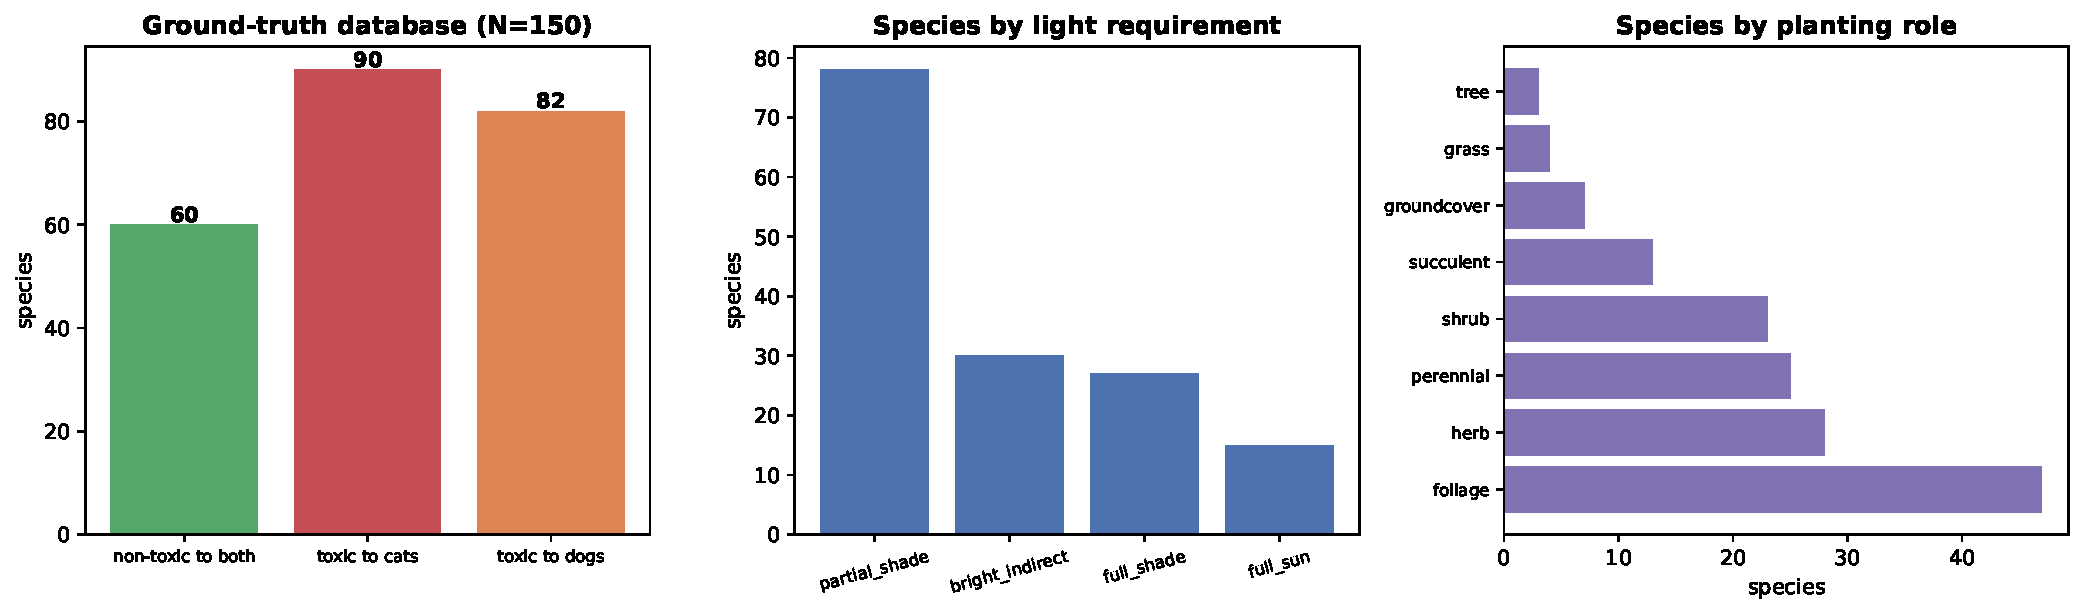
\includegraphics[width=0.62\linewidth]{fig4_db_composition.pdf}
  \caption{Composition of the ground-truth database by light requirement,
  moisture requirement and planting role.}
  \label{fig:db}
\end{figure}

\subsection{Why this data is suitable for evaluation}

The toxicity label is a \emph{binary, expert-certified} fact with an
authoritative source and a stable URL per row, so scoring has no
inter-annotator ambiguity. The horticultural labels make the task a genuine
two-constraint optimisation rather than a toy task: a species can be perfectly
safe and still be a poor choice for a dry, north-facing balcony. The database
contains a deliberate balance of safe and unsafe species, which is what makes
the safety metric discriminative rather than trivially satisfied.

\subsection{Limitations of the data}

The database covers 150 species, not the full ASPCA list of more than a
thousand; the ASPCA taxonomy is species-level and does not distinguish
cultivars; only cats and dogs are covered, although ASPCA also lists horses;
and the moisture values are curated rather than machine-extracted.

\section{Experiment Setting, Baselines and Performance}

\subsection{Evaluation tasks}

The benchmark consists of 25 realistic household scenarios, each a
natural-language brief plus a structured ground truth of the site conditions
and the household pets. The scenarios cross 4 light classes (deep shade,
partial shade, bright indirect, full sun), 3 moisture classes and 4 pet
configurations (cat only, dog only, a multi-pet household, and a no-pet
control), covering 12 distinct light--moisture combinations.
\texttt{data/scenarios.csv} contains the full set, together with the
challenge each scenario is designed to expose.

\subsection{Methods compared}

\begin{itemize}
  \item \textbf{Baseline 1 --- direct zero-shot LLM.} One turn, no tools, no
    database: the model relies entirely on parametric memory.
  \item \textbf{Baseline 2 --- naive keyword RAG.} BM25 retrieval over the
    same catalogue, \emph{without} any toxicological filtering, followed by
    one synthesis turn. This baseline isolates the contribution of grounding
    from the contribution of safety filtering.
  \item \textbf{Proposed --- dual-constraint agent.} The workflow of
    Section~2, with the deterministic filter, the relaxation ladder and the
    audit loop.
\end{itemize}

\subsection{Metrics}

All metrics are computed by deterministic Python code against the same
ground-truth database; the evaluator never asks the model whether it was
right. (1) \emph{Pet safety compliance}: share of recommended plants
non-toxic to every household pet. (2) \emph{Horticultural viability}: share
matching the site's light and moisture. (3) \emph{Dual-constraint accuracy}:
share satisfying both simultaneously. (4) \emph{Design completeness}: a
fifteen-item binary rubric (Section~\ref{sec:rubric}) over spatial zoning,
combination logic, care instructions, care cautions, pet-safety notes and
coverage; reported both as a 0--15 score and as a 0--5 core. (5)
\emph{Out-of-database rate}: share of recommended plants that are not in the
curated catalogue, i.e. hallucinated species.

Every one of these is computed against the tiered evidence of
Section~\ref{sec:resolving}. Two are reported in two versions: the
\emph{conservative} safety rate counts a species as safe only when the ASPCA
certifies it, while the \emph{resolved} rate additionally admits the
ASPCA-aligned secondary source and is restricted to species that could be
judged at all. The conservative version carries the safety claim, the
resolved version is the fair comparison between methods, and the gap is
reported so that no reader has to guess which is which. Three further
counters make the provenance auditable: species outside the curated
catalogue, species no source could resolve, and species judgeable for
viability.

\subsection{Results}

\begin{table}[!ht]
\centering
\begin{tabular}{lcccccc}
\toprule
Method & Safety $\uparrow$ & Safety* $\uparrow$ & Viability $\uparrow$ &
Dual $\uparrow$ & Completeness (0--15) $\uparrow$ & Out-of-DB $\downarrow$ \\
\midrule
Baseline 1 (zero-shot) & \todo{} & \todo{} & \todo{} & \todo{} & \todo{} & \todo{} \\
Baseline 2 (naive RAG) & \todo{} & \todo{} & \todo{} & \todo{} & \todo{} & \todo{} \\
\textbf{Proposed (agent)} & \todo{} & \todo{} & \todo{} & \todo{} & \todo{} & \todo{} \\
\bottomrule
\end{tabular}

\vspace{1mm}
{\footnotesize Safety is the conservative rate (ASPCA-certified only); Safety$^*$ is the
resolved rate over the species that could be judged at all
(Section~\ref{sec:resolving}). \todo{Insert both and state the difference
explicitly in the text.}}

\vspace{2mm}
\begin{tabular}{lccccc}
\toprule
& & & & \multicolumn{2}{c}{Design Completeness} \\
\cmidrule(lr){5-6}
Method & zones A1--A3 & care C2--C3 & & core (0--5) & mean missing items \\
\midrule
Baseline 1 (zero-shot) & \todo{} & \todo{} &  & \todo{} & \todo{} \\
Baseline 2 (naive RAG) & \todo{} & \todo{} &  & \todo{} & \todo{} \\
\textbf{Proposed (agent)} & \todo{} & \todo{} &  & \todo{} & \todo{} \\
\bottomrule
\end{tabular}
\caption{Main results over the 25 benchmark scenarios. Fill from
\texttt{results/runs/<provider>\_\_<model>/summary.csv}.}
\end{table}

\begin{figure}[t]
  \centering
  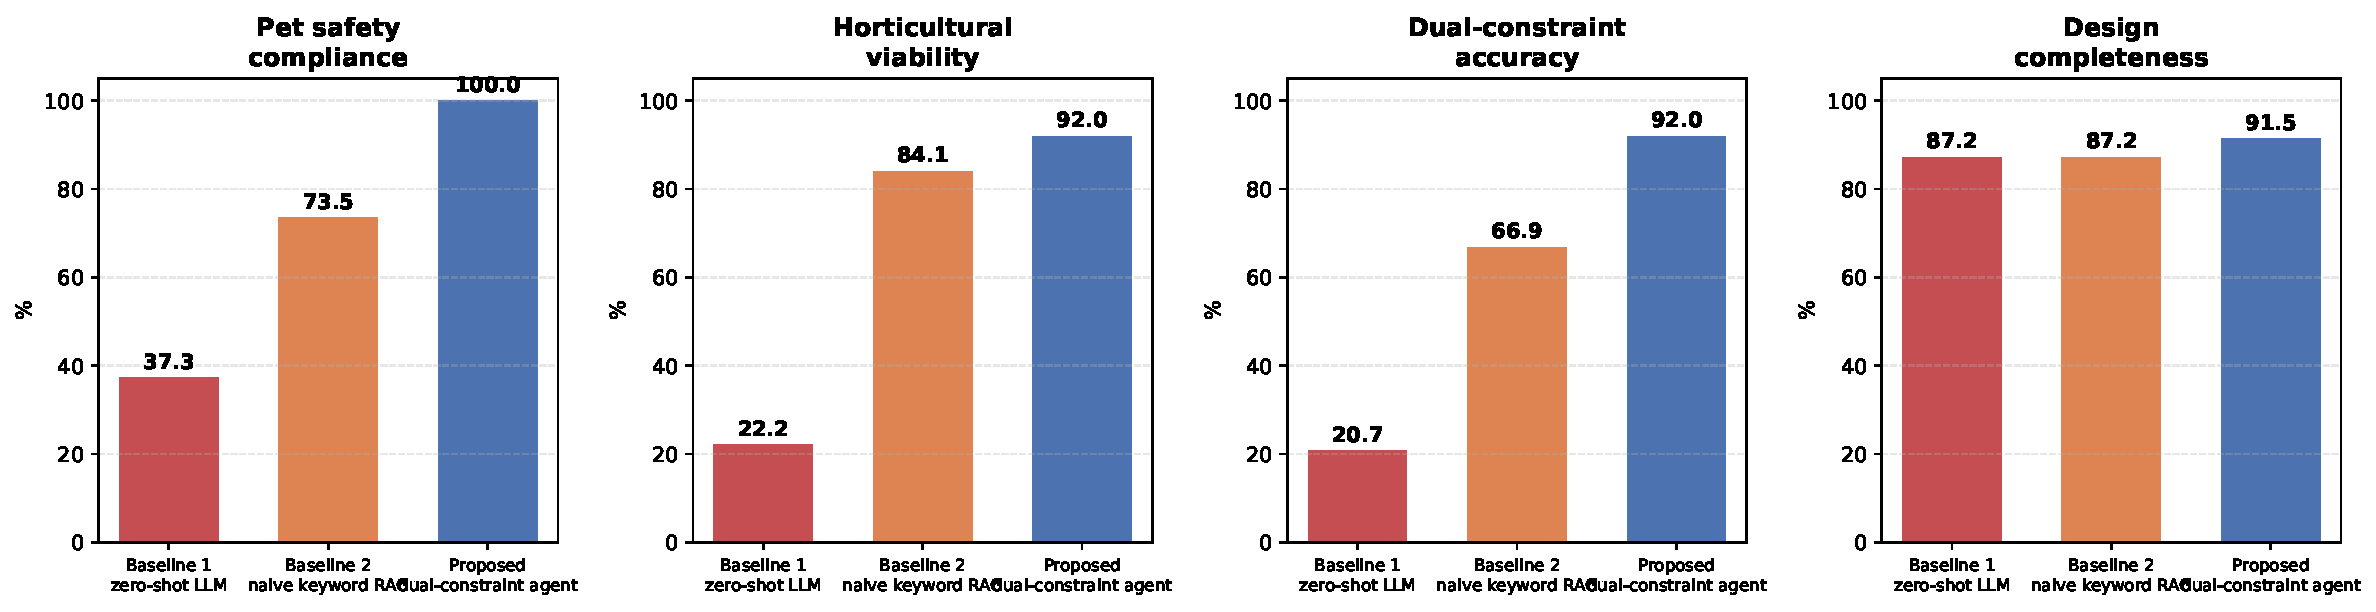
\includegraphics[width=0.58\linewidth]{fig1_main_metrics.pdf}
  \caption{The four headline metrics for the three methods.}
  \label{fig:main}
\end{figure}

\begin{figure}[t]
  \centering
  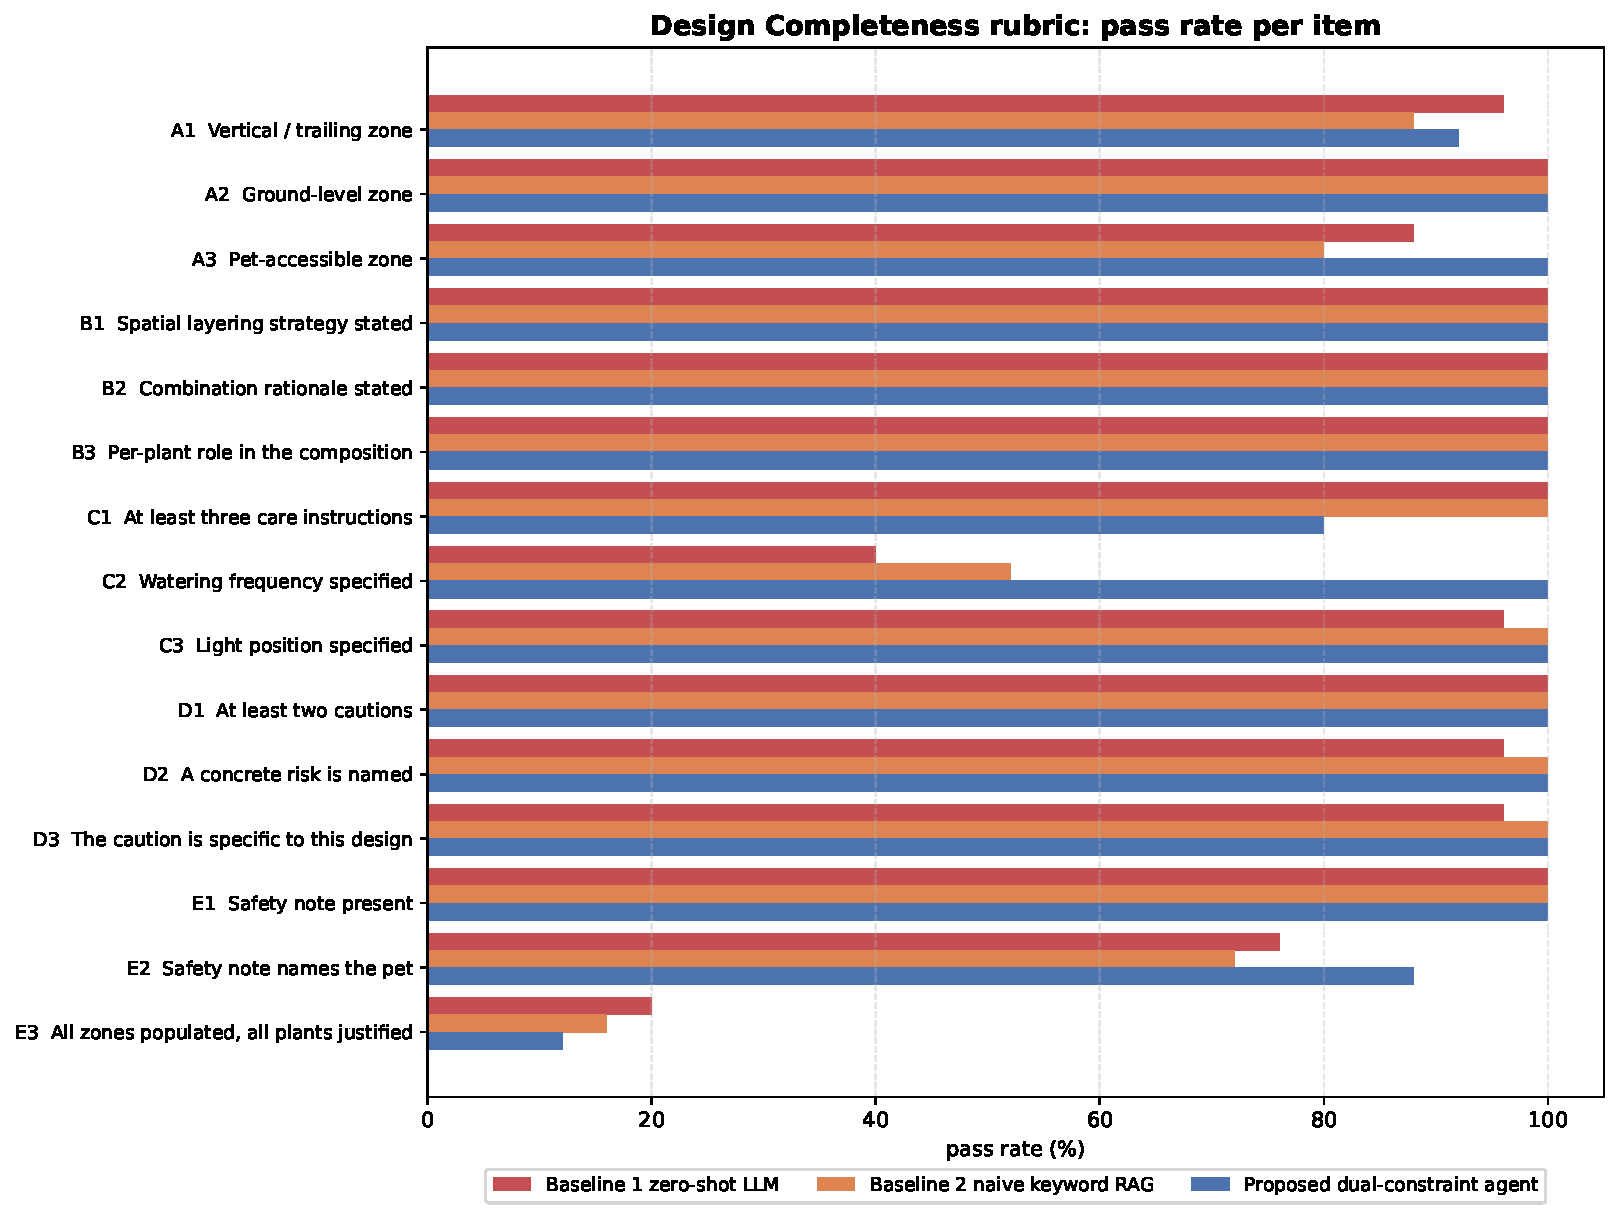
\includegraphics[width=0.49\linewidth]{fig6_rubric_items.pdf}\hfill
  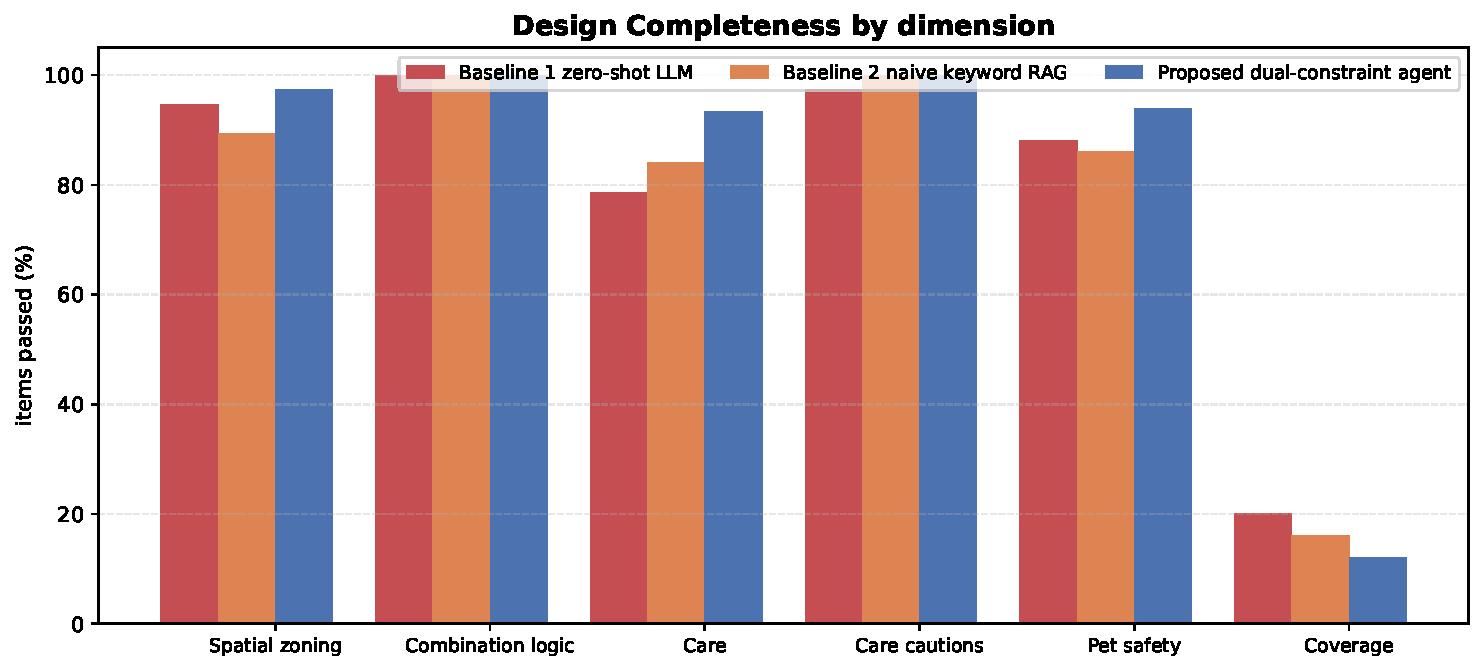
\includegraphics[width=0.49\linewidth]{fig7_completeness_dimensions.pdf}
  \caption{Design Completeness for the three methods: pass rate of every rubric
  item (left), which shows \emph{which} design knowledge each method lacks,
  and score by dimension (right), which groups them into spatial zoning,
  combination logic, care, care cautions and pet-safety reasoning.}
  \label{fig:rubric}
\end{figure}

\subsection{Analysis}

\todo{Discuss: (i) why the agent's safety rate is exactly 1.0 --- the filter
is deterministic, so the model is never given the opportunity to choose an
unsafe species, rather than the model being "more careful"; (ii) why the
baselines' viability is competitive while their safety is not --- the two
constraint families are independent, and grounding alone fixes only one of
them; (iii) the incremental value of retrieval (B1 vs B2) and of negative
filtering (B2 vs proposed); (iv) a concrete failure case, e.g. a zero-shot
design in which a true lily was proposed for a cat household.}

\paragraph{Design quality is a separate axis from safety.}
The completeness rubric separates two things that are usually conflated. A
design can be perfectly safe and still be useless: a list of six
non-toxic plants with no spatial structure, no maintenance advice and no
warning about the watering regime is safe and still not a planting scheme.
Figure~\ref{fig:rubric} shows that the baselines are not uniformly weaker:
they usually satisfy the items that any competent LLM produces (a zone
structure, a justification per plant, a list of care tasks) and lose points
on the items that require the model to reason about the \emph{design as a
whole} --- a reachable pet zone, cautions that name a specific plant, and a
safety note that names the animal in question. These are exactly the items
a user would notice in a delivered scheme.

The completeness repair loop matters here. Because the rubric is
deterministic, the agent can be told precisely which items it failed, so the
gain in completeness (Table~1) is produced by a verified mechanism rather
than by a more elaborate prompt. The same argument applies to design
quality: \emph{a property that can be checked should be checked by code, and
the failure handed back to the model as an explicit, actionable list}.

\section{Discussions}

\textbf{What the results mean.} The safety gain is architectural, not a prompt
effect: the candidate pool is produced by a set operation over an explicit
table, so the agent's pet-safety compliance is a property of the database
rather than of the language model. This also explains why naive RAG improves
viability but not safety: retrieval grounds the model in the catalogue without
stopping it choosing a toxic entry of it.

\textbf{Limitations.} Only cats and dogs are modelled; the benchmark has 25
scenarios; and constraint extraction is itself an LLM call, so a mis-parsed
brief propagates into the candidate pool. The ladder mitigates but does not
remove this: it guarantees safety, not optimality. Results are
model-version specific, although the safety floor is not.

\textbf{Outlook.} Extensions include iterative tool use, explicit provenance,
hybrid retrieval to scale the catalogue, and a wider pet profile.

\textbf{Conclusion.} In safety-critical applications the useful question is
not which model is cleverest but which decisions may remain unverifiable.
Moving every checkable constraint out of the model and into an auditable
tool makes a moderate LLM reliable where a stronger LLM is not; the value of
an agentic workflow lies in placing the right computation.

\clearpage
\begin{thebibliography}{99}
\bibitem{aspca}
ASPCA Animal Poison Control. \emph{Toxic and Non-Toxic Plants}.
\url{https://www.aspca.org/pet-care/animal-poison-control/toxic-and-non-toxic-plants}

\bibitem{ncstate}
NC State Extension. \emph{Plant Toolbox}.
\url{https://plants.ces.ncsu.edu/}

\bibitem{mobot}
Missouri Botanical Garden. \emph{Plant Finder}.
\url{https://www.missouribotanicalgarden.org/PlantFinder/}

\bibitem{gemini}
Google AI for Developers. \emph{Gemini API documentation}.
\url{https://ai.google.dev/gemini-api/docs}

\bibitem{deepseek}
DeepSeek. \emph{API Documentation}.
\url{https://api-docs.deepseek.com/}

\bibitem{webagents}
Ning, L., et al. (2025). \emph{A Survey of WebAgents: Towards Next-Generation
AI Agents for Web Automation with Large Foundation Models}. arXiv:2503.23350.

\bibitem{jiuwen}
openJiuwen Agent Platform. \url{https://openjiuwen.com/en/}

\bibitem{bm25}
Robertson, S., Zaragoza, H. (2009). \emph{The Probabilistic Relevance Framework:
BM25 and Beyond}. Foundations and Trends in Information Retrieval, 3(4).

\bibitem{schick2023}
Schick, T., et al. (2023). \emph{Toolformer: Language Models Can Teach
Themselves to Use Tools}. NeurIPS 2023.

\bibitem{yao2023}
Yao, S., et al. (2023). \emph{ReAct: Synergizing Reasoning and Acting in
Language Models}. ICLR 2023.

\bibitem{shinn2023}
Shinn, N., et al. (2023). \emph{Reflexion: Language Agents with Verbal
Reinforcement Learning}. NeurIPS 2023.

\bibitem{aspet}
ASPCA. \emph{Poison Control Factsheets and Toxic Plant List}.
\url{https://www.aspca.org/pet-care/animal-poison-control}

\end{thebibliography}

\end{document}
